% THIS IS SIGPROC-SP.TEX - VERSION 3.1
% WORKS WITH V3.2SP OF ACM_PROC_ARTICLE-SP.CLS
% APRIL 2009
%
% It is an example file showing how to use the 'acm_proc_article-sp.cls' V3.2SP
% LaTeX2e document class file for Conference Proceedings submissions.
% ----------------------------------------------------------------------------------------------------------------
% This .tex file (and associated .cls V3.2SP) *DOES NOT* produce:
%       1) The Permission Statement
%       2) The Conference (location) Info information
%       3) The Copyright Line with ACM data
%       4) Page numbering
% ---------------------------------------------------------------------------------------------------------------
% It is an example which *does* use the .bib file (from which the .bbl file
% is produced).
% REMEMBER HOWEVER: After having produced the .bbl file,
% and prior to final submission,
% you need to 'insert'  your .bbl file into your source .tex file so as to provide
% ONE 'self-contained' source file.
%
% Questions regarding SIGS should be sent to
% Adrienne Griscti ---> griscti@acm.org
%
% Questions/suggestions regarding the guidelines, .tex and .cls files, etc. to
% Gerald Murray ---> murray@hq.acm.org
%
% For tracking purposes - this is V3.1SP - APRIL 2009

\documentclass{acm_proc_article-sp}

\begin{document}

\title{Bar Dude \\ An Interactive Bar}
%\subtitle{[Extended Abstract]
%\titlenote{A full version of this paper is available as
%\textit{Author's Guide to Preparing ACM SIG Proceedings Using
%\LaTeX$2_\epsilon$\ and BibTeX} at
%\texttt{www.acm.org/eaddress.htm}}}
%
% You need the command \numberofauthors to handle the 'placement
% and alignment' of the authors beneath the title.
%
% For aesthetic reasons, we recommend 'three authors at a time'
% i.e. three 'name/affiliation blocks' be placed beneath the title.
%
% NOTE: You are NOT restricted in how many 'rows' of
% "name/affiliations" may appear. We just ask that you restrict
% the number of 'columns' to three.
%
% Because of the available 'opening page real-estate'
% we ask you to refrain from putting more than six authors
% (two rows with three columns) beneath the article title.
% More than six makes the first-page appear very cluttered indeed.
%
% Use the \alignauthor commands to handle the names
% and affiliations for an 'aesthetic maximum' of six authors.
% Add names, affiliations, addresses for
% the seventh etc. author(s) as the argument for the
% \additionalauthors command.
% These 'additional authors' will be output/set for you
% without further effort on your part as the last section in
% the body of your article BEFORE References or any Appendices.

\numberofauthors{4} %  in this sample file, there are a *total*
% of EIGHT authors. SIX appear on the 'first-page' (for formatting
% reasons) and the remaining two appear in the \additionalauthors section.
%
\author{
% You can go ahead and credit any number of authors here,
% e.g. one 'row of three' or two rows (consisting of one row of three
% and a second row of one, two or three).
%
% The command \alignauthor (no curly braces needed) should
% precede each author name, affiliation/snail-mail address and
% e-mail address. Additionally, tag each line of
% affiliation/address with \affaddr, and tag the
% e-mail address with \email.
%
% 1st. author
\alignauthor
Nicolas Erbach\\
       %\affaddr{1932 Wallamaloo Lane}\\
       %\affaddr{Wallamaloo, New Zealand}\\
       \email{s9nierba@stud.uni-saarland.de}
% 2nd. author
\alignauthor
Tobias Kiefer\\
       %\affaddr{Institute for Clarity in Documentation}\\
       %\affaddr{P.O. Box 1212}\\
       %\affaddr{Dublin, Ohio 43017-6221}\\
       \email{s9tskief@stud.uni-saarland.de}
% 3rd. author
\alignauthor Maike Maas\\
      % \affaddr{The Th{\o}rv{\"a}ld Group}\\
      % \affaddr{1 Th{\o}rv{\"a}ld Circle}\\
       % \affaddr{Hekla, Iceland}\\
       \email{s9memaas@stud.uni-saarland.de}
\and  % use '\and' if you need 'another row' of author names
% 4th. author
\alignauthor Manuel Zapp\\
       %\affaddr{Brookhaven Laboratories}\\
       %\affaddr{Brookhaven National Lab}\\
       %\affaddr{P.O. Box 5000}\\
       \email{s9mazapp@stud.uni-saarland.de}
}
% There's nothing stopping you putting the seventh, eighth, etc.
% author on the opening page (as the 'third row') but we ask,
% for aesthetic reasons that you place these 'additional authors'
% in the \additional authors block, viz.
%\additionalauthors{Additional authors: John Smith (The Th{\o}rv{\"a}ld Group,
%email: {\texttt{jsmith@affiliation.org}}) and Julius P.~Kumquat
%(The Kumquat Consortium, email: {\texttt{jpkumquat@consortium.net}}).}
\date{25 September 2015}
% Just remember to make sure that the TOTAL number of authors
% is the number that will appear on the first page PLUS the
% number that will appear in the \additionalauthors section.

\maketitle
\begin{abstract}
%This paper provides a sample of a \LaTeX\ document which conforms to
%the formatting guidelines for ACM SIG Proceedings.
%It complements the document \textit{Author's Guide to Preparing
%ACM SIG Proceedings Using \LaTeX$2_\epsilon$\ and Bib\TeX}. This
%source file has been written with the intention of being
%compiled under \LaTeX$2_\epsilon$\ and BibTeX.
%
%The developers have tried to include every imaginable sort
%of ``bells and whistles", such as a subtitle, footnotes on
%title, subtitle and authors, as well as in the text, and
%every optional component (e.g. Acknowledgments, Additional
%Authors, Appendices), not to mention examples of
%equations, theorems, tables and figures.
%
%To make best use of this sample document, run it through \LaTeX\
%and BibTeX, and compare this source code with the printed
%output produced by the dvi file.
\end{abstract}

% A category with the (minimum) three required fields
%\category{H.4}{Information Systems Applications}{Miscellaneous}
%A category including the fourth, optional field follows...
%\category{D.2.8}{Software Engineering}{Metrics}[complexity measures, performance measures]

%\terms{Theory}

%\keywords{ACM proceedings, \LaTeX, text tagging} % NOT required for Proceedings

\section{Introduction}
%The \textit{proceedings} are the records of a conference.
%ACM seeks to give these conference by-products a uniform,
%high-quality appearance.  To do this, ACM has some rigid
%requirements for the format of the proceedings documents: there
%is a specified format (balanced  double columns), a specified
%set of fonts (Arial or Helvetica and Times Roman) in
%certain specified sizes (for instance, 9 point for body copy),
%a specified live area (18 $\times$ 23.5 cm [7" $\times$ 9.25"]) centered on
%the page, specified size of margins (1.9 cm [0.75"]) top, (2.54 cm [1"]) bottom
%and (1.9 cm [.75"]) left and right; specified column width
%(8.45 cm [3.33"]) and gutter size (.83 cm [.33"]).
%
%The good news is, with only a handful of manual
%settings\footnote{Two of these, the {\texttt{\char'134 numberofauthors}}
%and {\texttt{\char'134 alignauthor}} commands, you have
%already used; another, {\texttt{\char'134 balancecolumns}}, will
%be used in your very last run of \LaTeX\ to ensure
%balanced column heights on the last page.}, the \LaTeX\ document
%class file handles all of this for you.
%
%The remainder of this document is concerned with showing, in
%the context of an ``actual'' document, the \LaTeX\ commands
%specifically available for denoting the structure of a
%proceedings paper, rather than with giving rigorous descriptions
%or explanations of such commands.

\section{Concept}
\subsection{Idea}
The idea behind Bar Dude is a cocktail bar that guides people through the single steps of mixing their favourite cocktails. In a first step you are able to choose a cocktail on the website of the bar by connecting to it with your smart phone or laptop. In a second step it supports each client by illuminating the ingredients of the cocktail he or she selected step by step and by giving clear advice when you put enough of the single ingredients into the cocktail.
\subsection{Approach}

\section{Hardware Construction}
\subsection{Woodwork}
After planning the rack and the shelves of the bar, we calculated the amount of wood we would need to build it. In a next step we had to cut the wood we bought into the right pieces. For the rounding of the rack bottom we contacted a local carpenter since we did not have the right instruments for doing this difficult cuts properly. The other small pieces were cut with a buzz saw as you can see in figure \ref{fig:cutting_wood}.

\begin{figure}[htbp] 
  \centering
     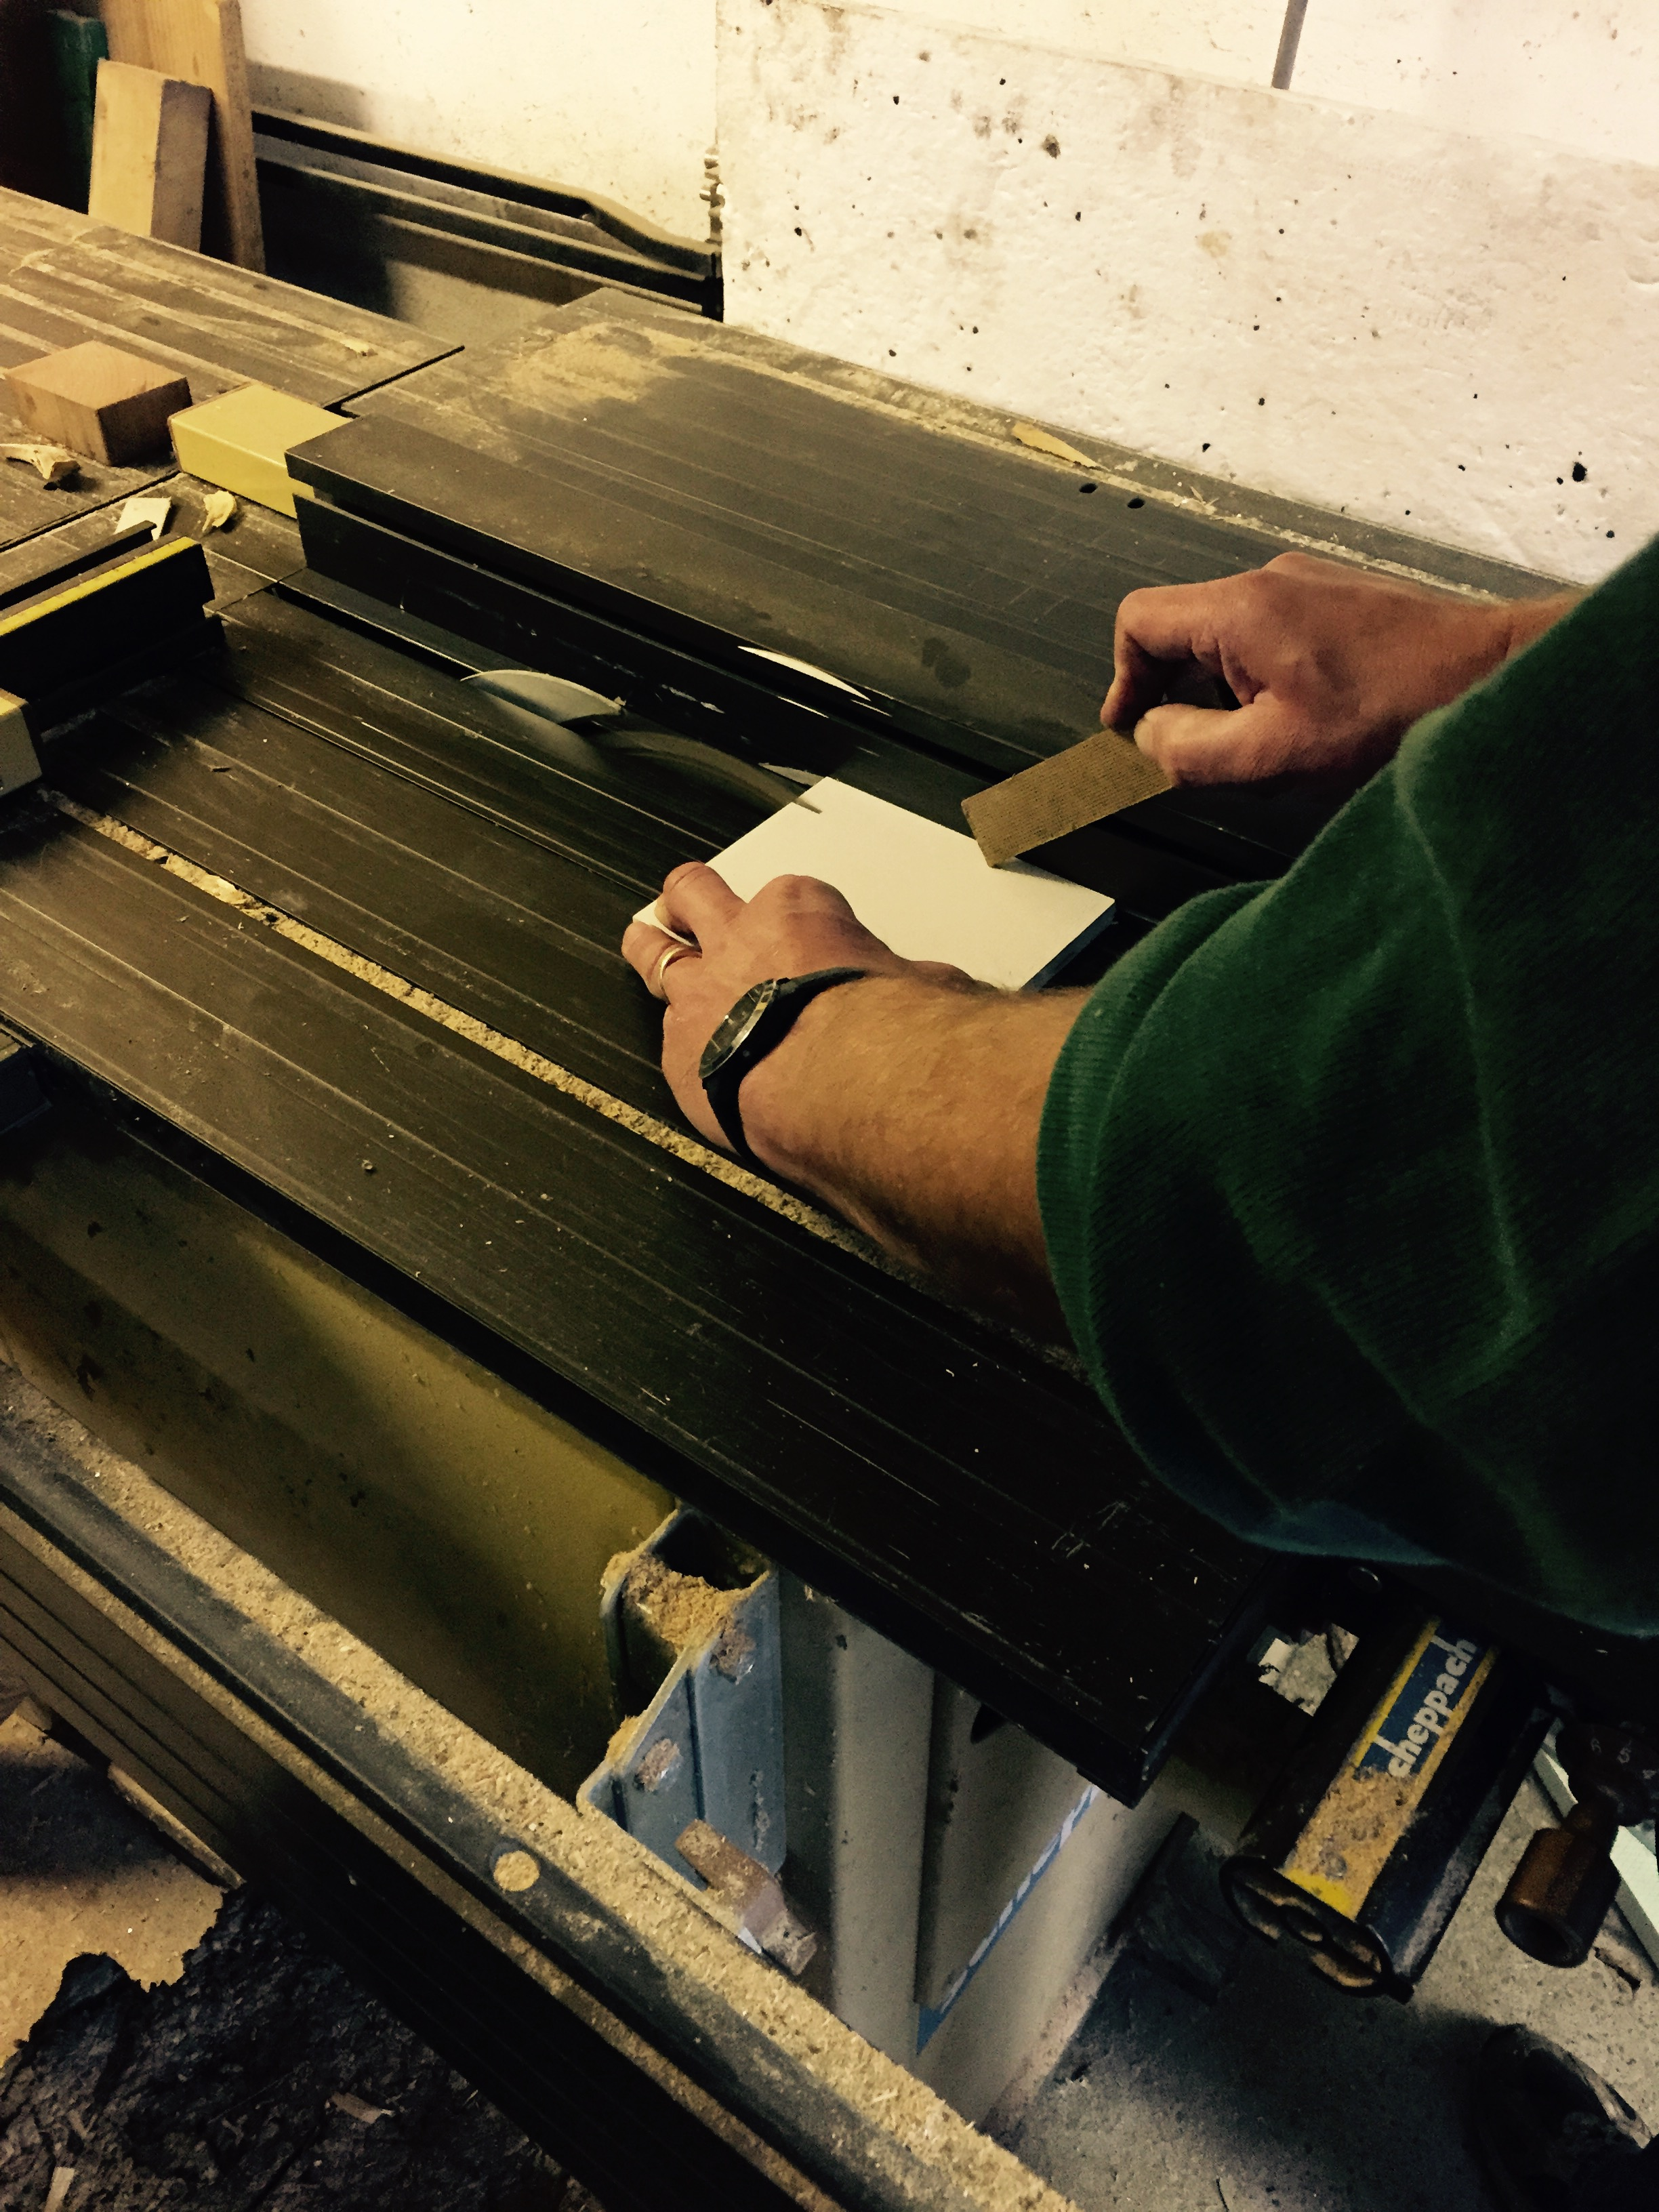
\includegraphics[width=0.5\linewidth]{pictures/cutting_wood.jpg}
  \caption{Cutting of the wood}
  \label{fig:cutting_wood}
\end{figure}

When all pieces of the rack were fitted, we started to assemble the rack. Therefore we used screws and wood glue so that the bar would keep stable. Figure \ref{fig:assembling} shows how the base plate is screwed together.

\begin{figure}[htbp] 
  \centering
     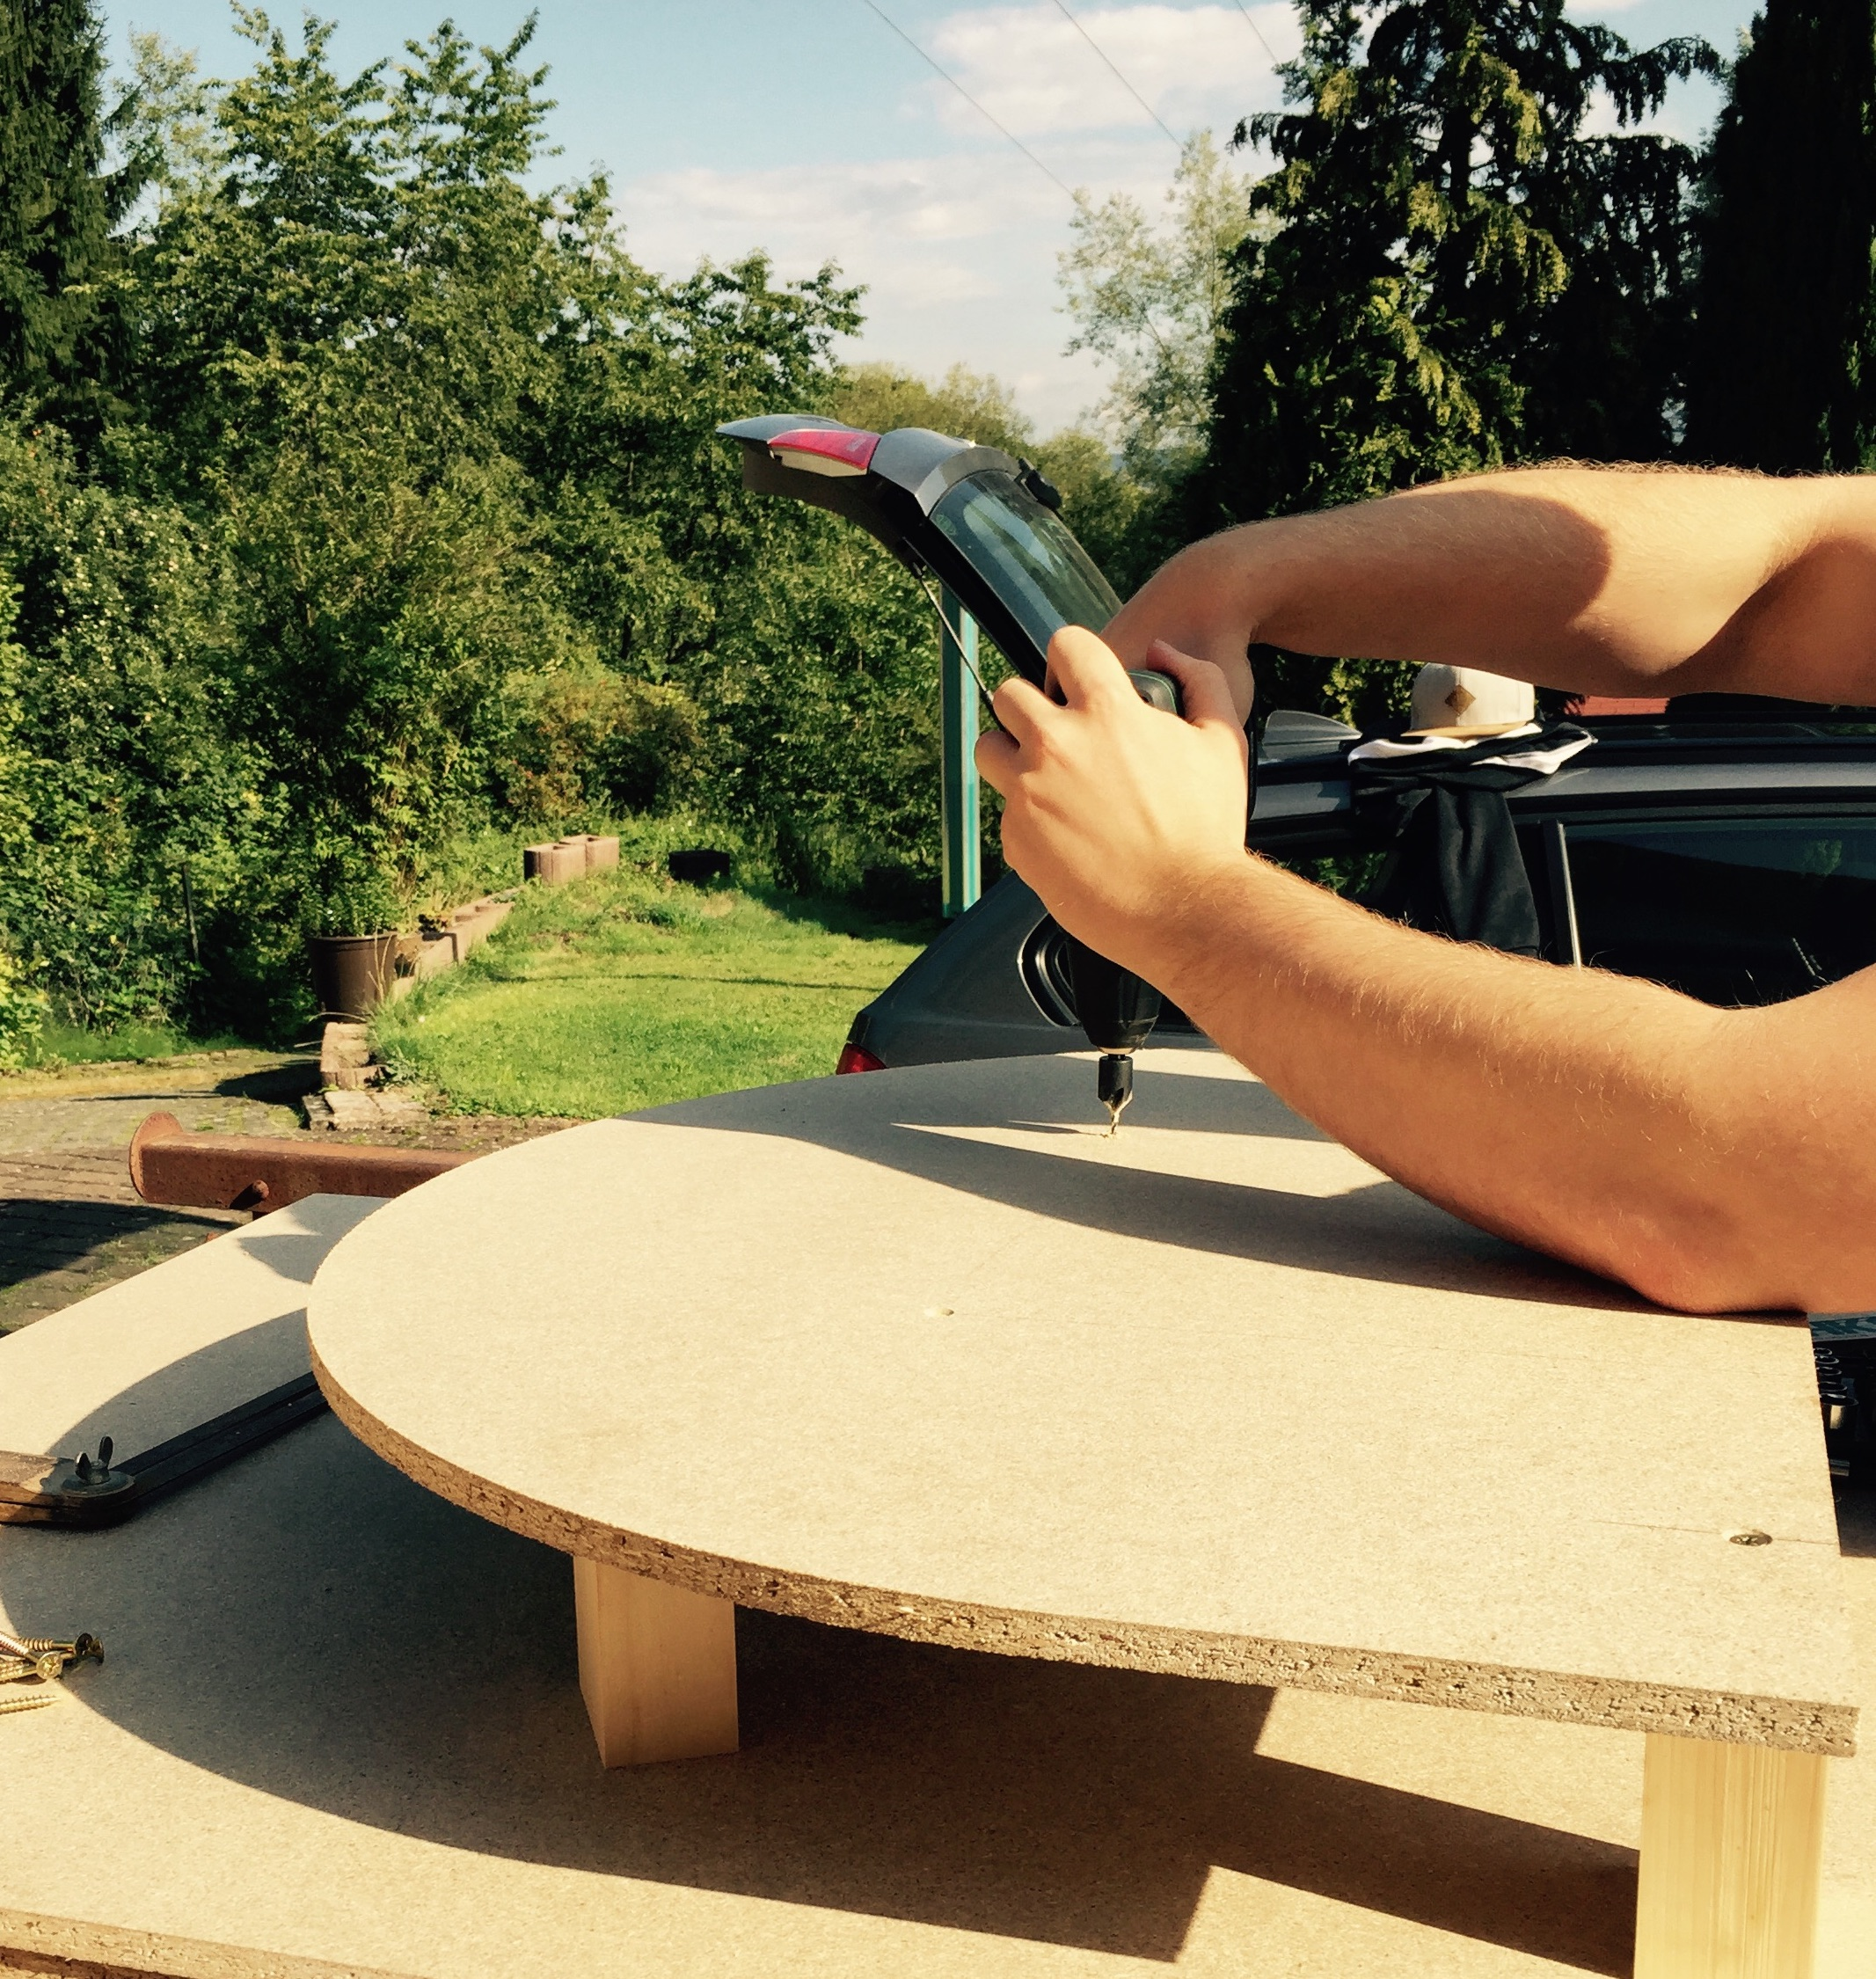
\includegraphics[width=0.5\linewidth]{pictures/assembling.jpg}
  \caption{Assembling of the rack}
  \label{fig:assembling}
\end{figure}

The finished framing of the rack is shown in figure \ref{fig:framing}. This picture also illustrates that we did the panelling between the two base plates with 4 mm poplar wood because this is to thin and flexible that it can be bend.

\begin{figure}[htbp] 
  \centering
     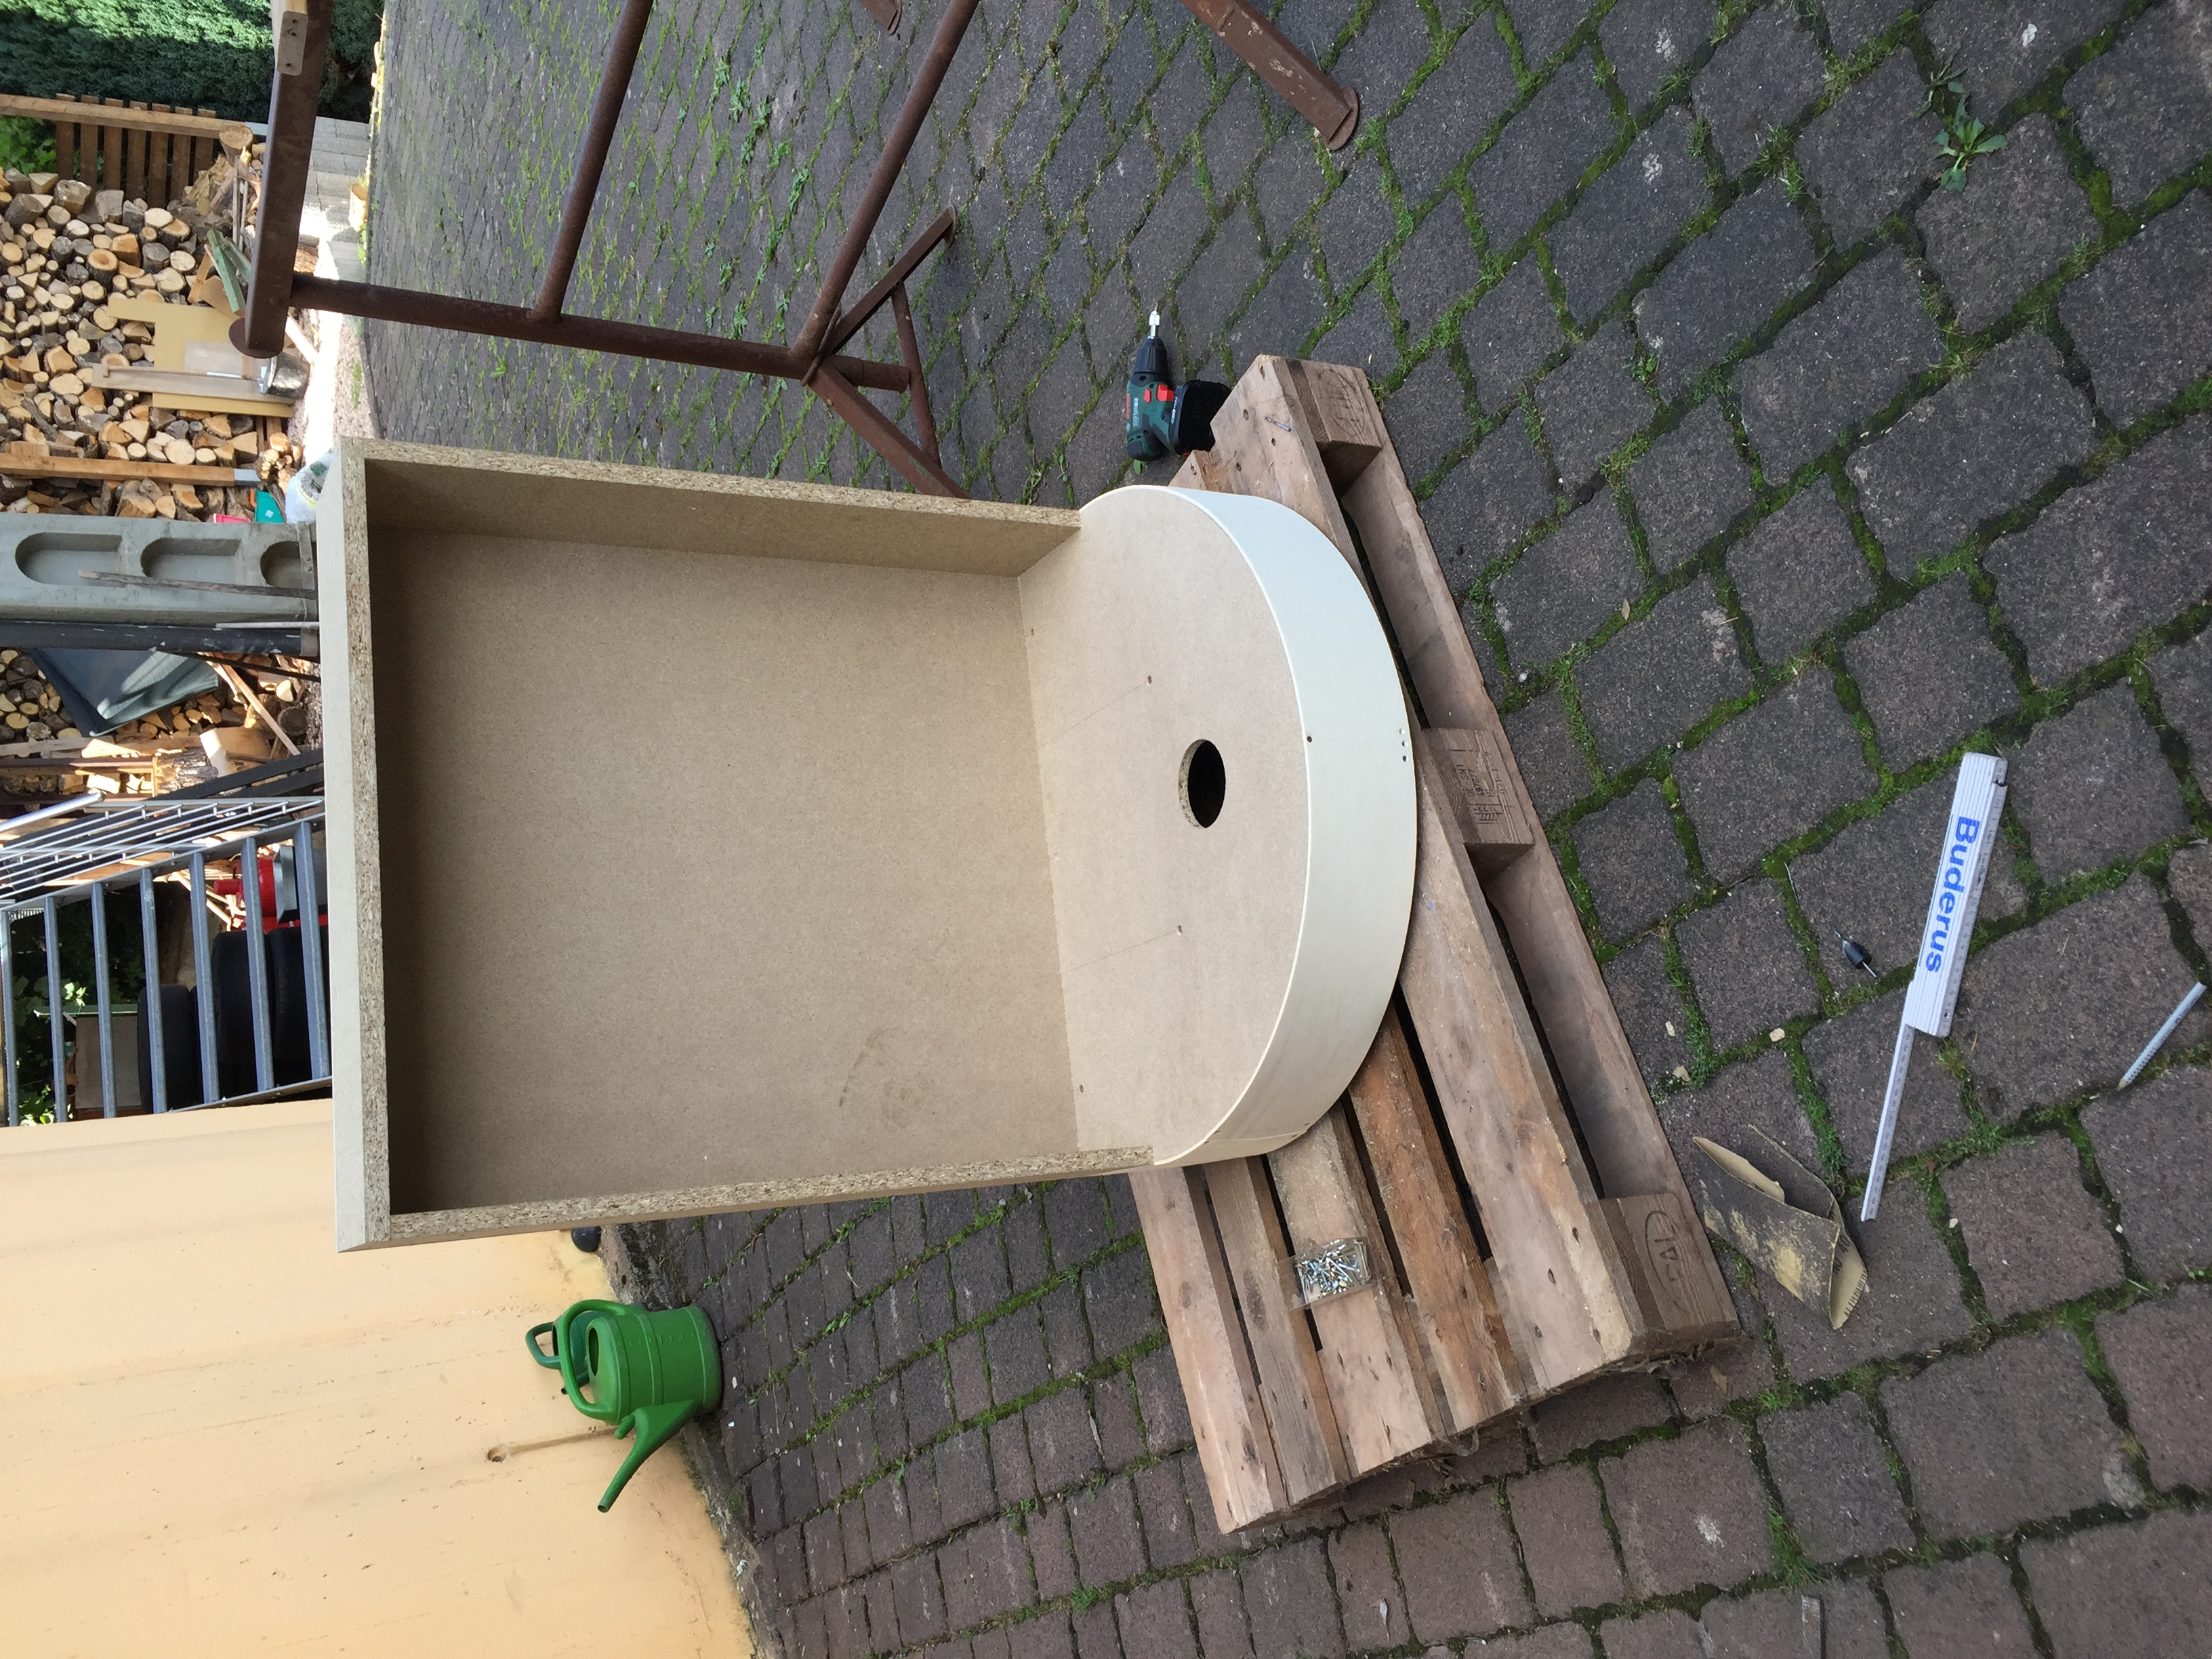
\includegraphics[width=0.6\linewidth, angle =270]{pictures/rack2.jpg}
  \caption{Framing of the rack}
  \label{fig:framing}
\end{figure}

For deriving a smooth surface of the rack, we filled all screw wholes with filler. Since we used plywood, we also filled the edges of the rack, so that it is easier to prime and paint the bar. 

\begin{figure}[htbp]  
  \centering
     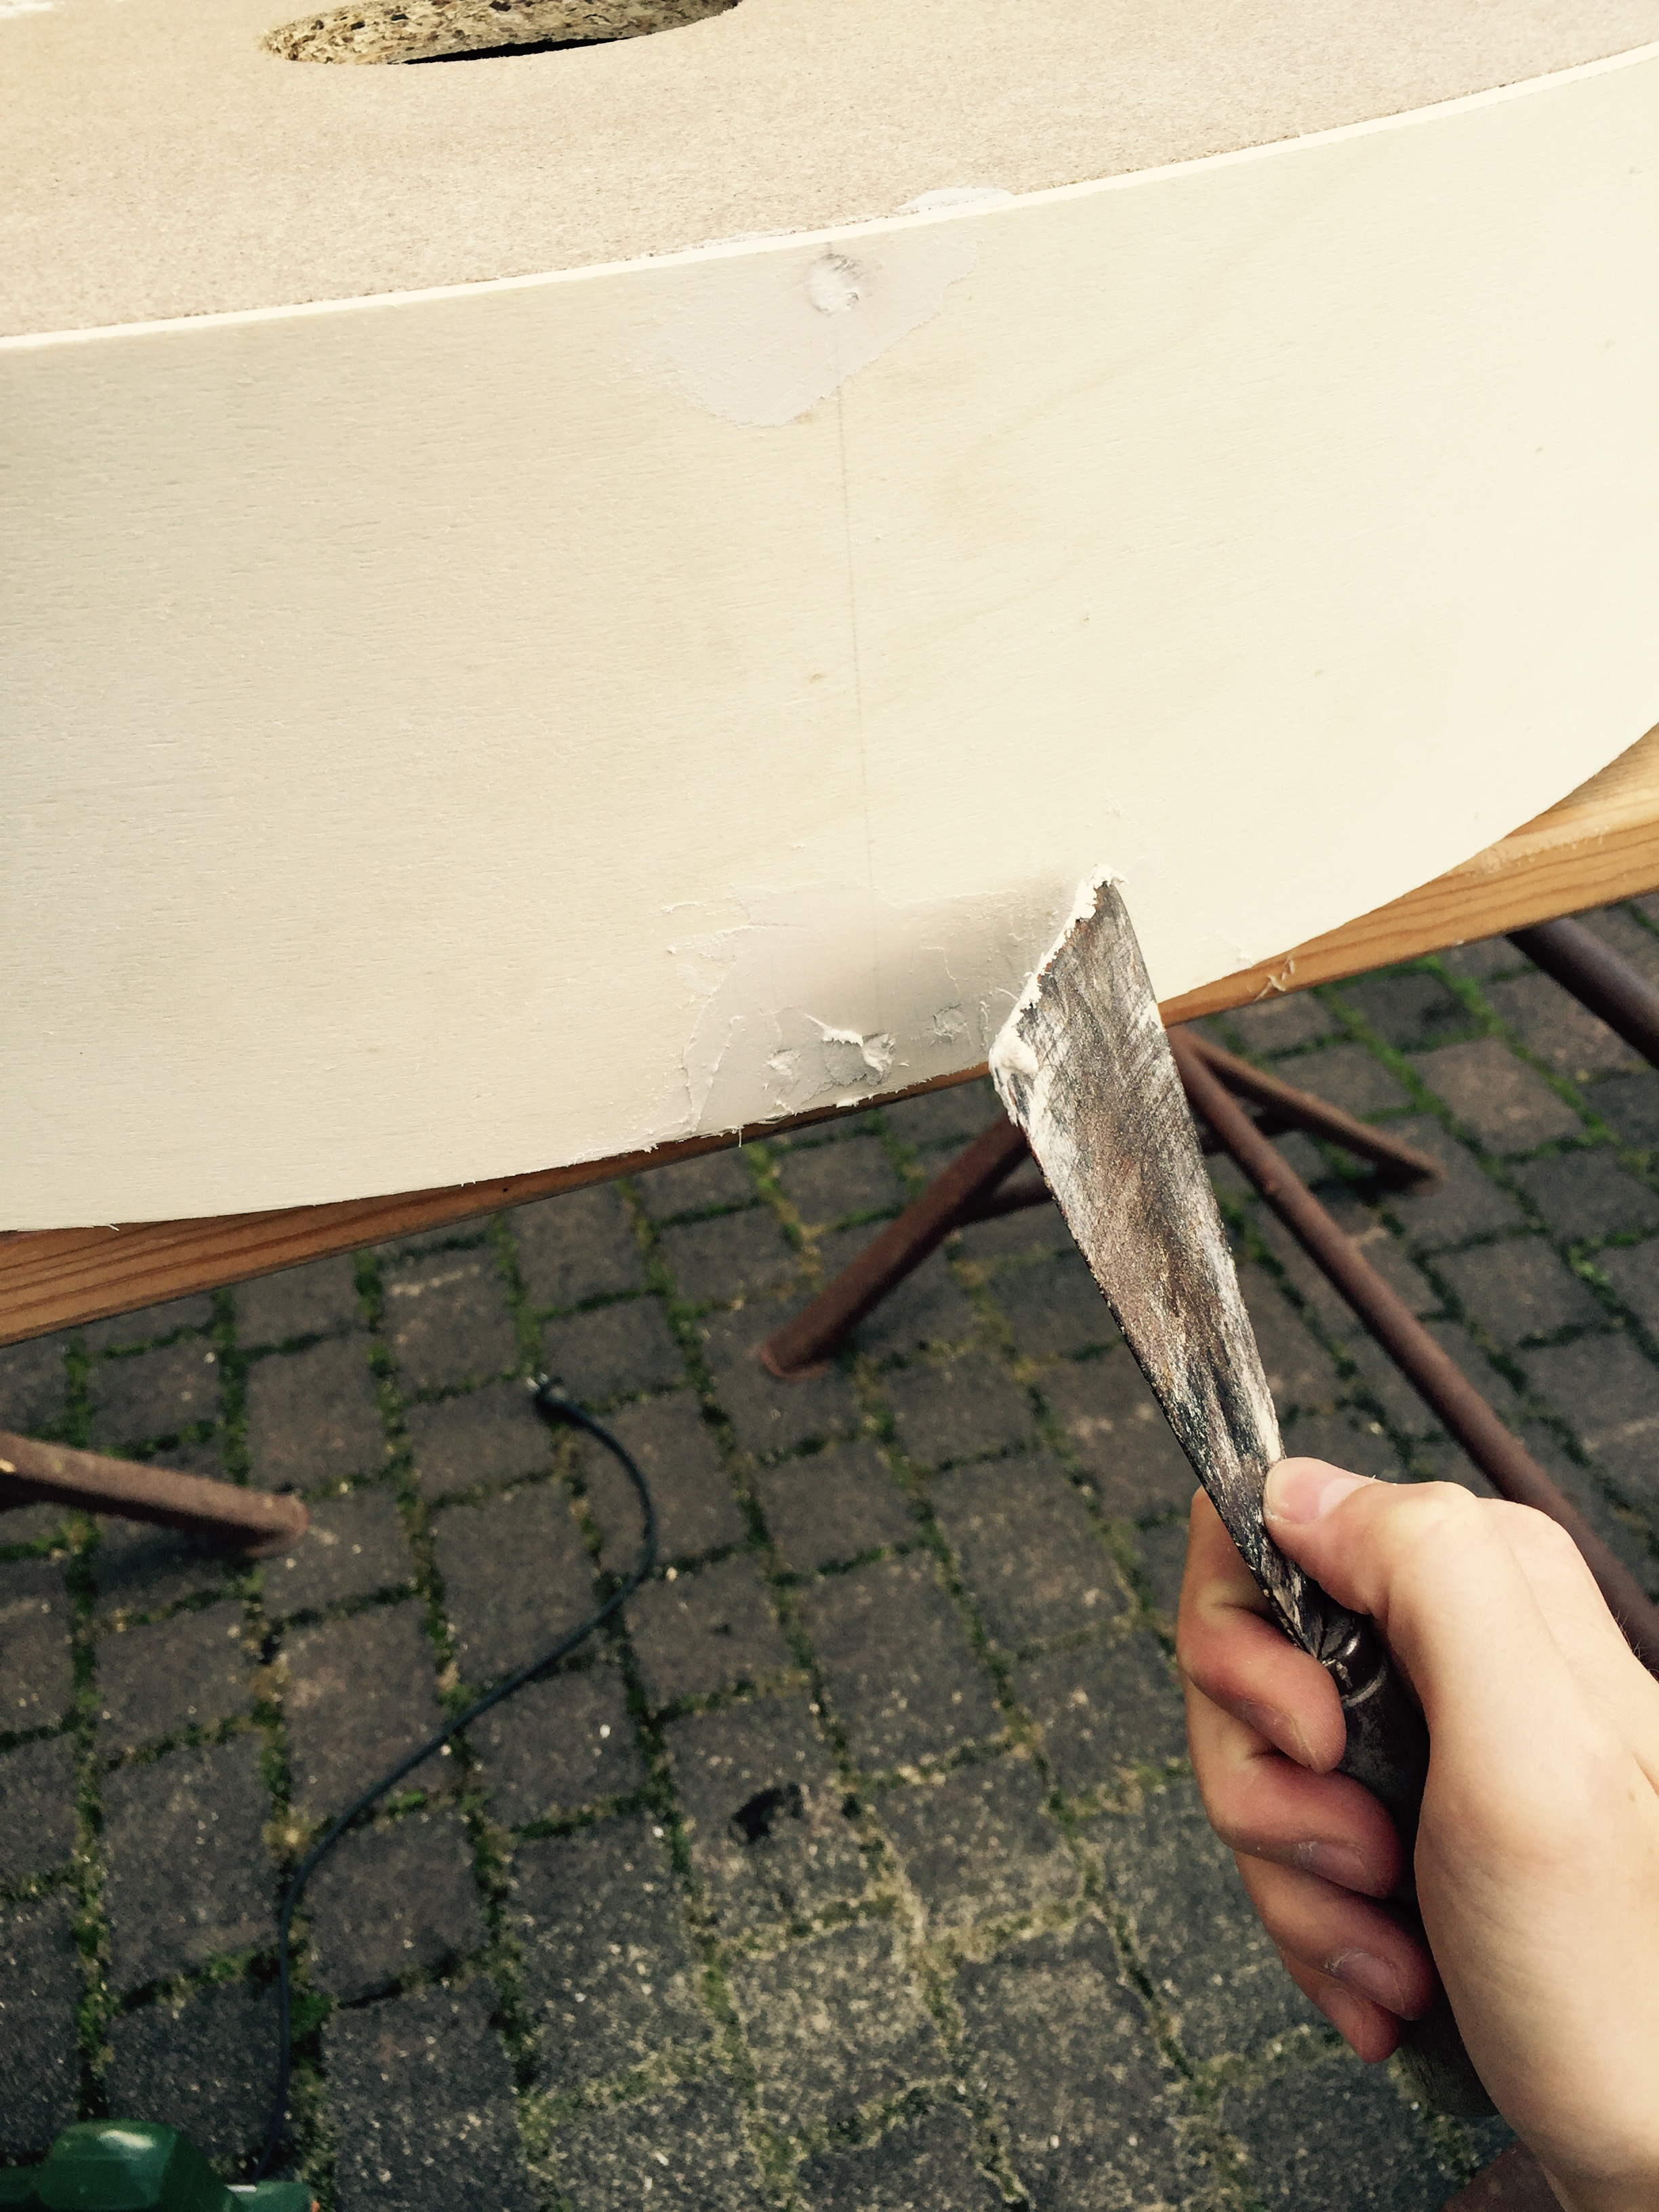
\includegraphics[width=0.5\linewidth]{pictures/filling.jpg}
  \caption{Filling of the screw wholes}
  \label{fig:filling}
\end{figure}

In a next step we polished the bar since had to remove the needless filler and roughen the wood. This work step can be seen in figure \ref{fig:polishing}
 
\begin{figure}[htbp] 
  \centering
     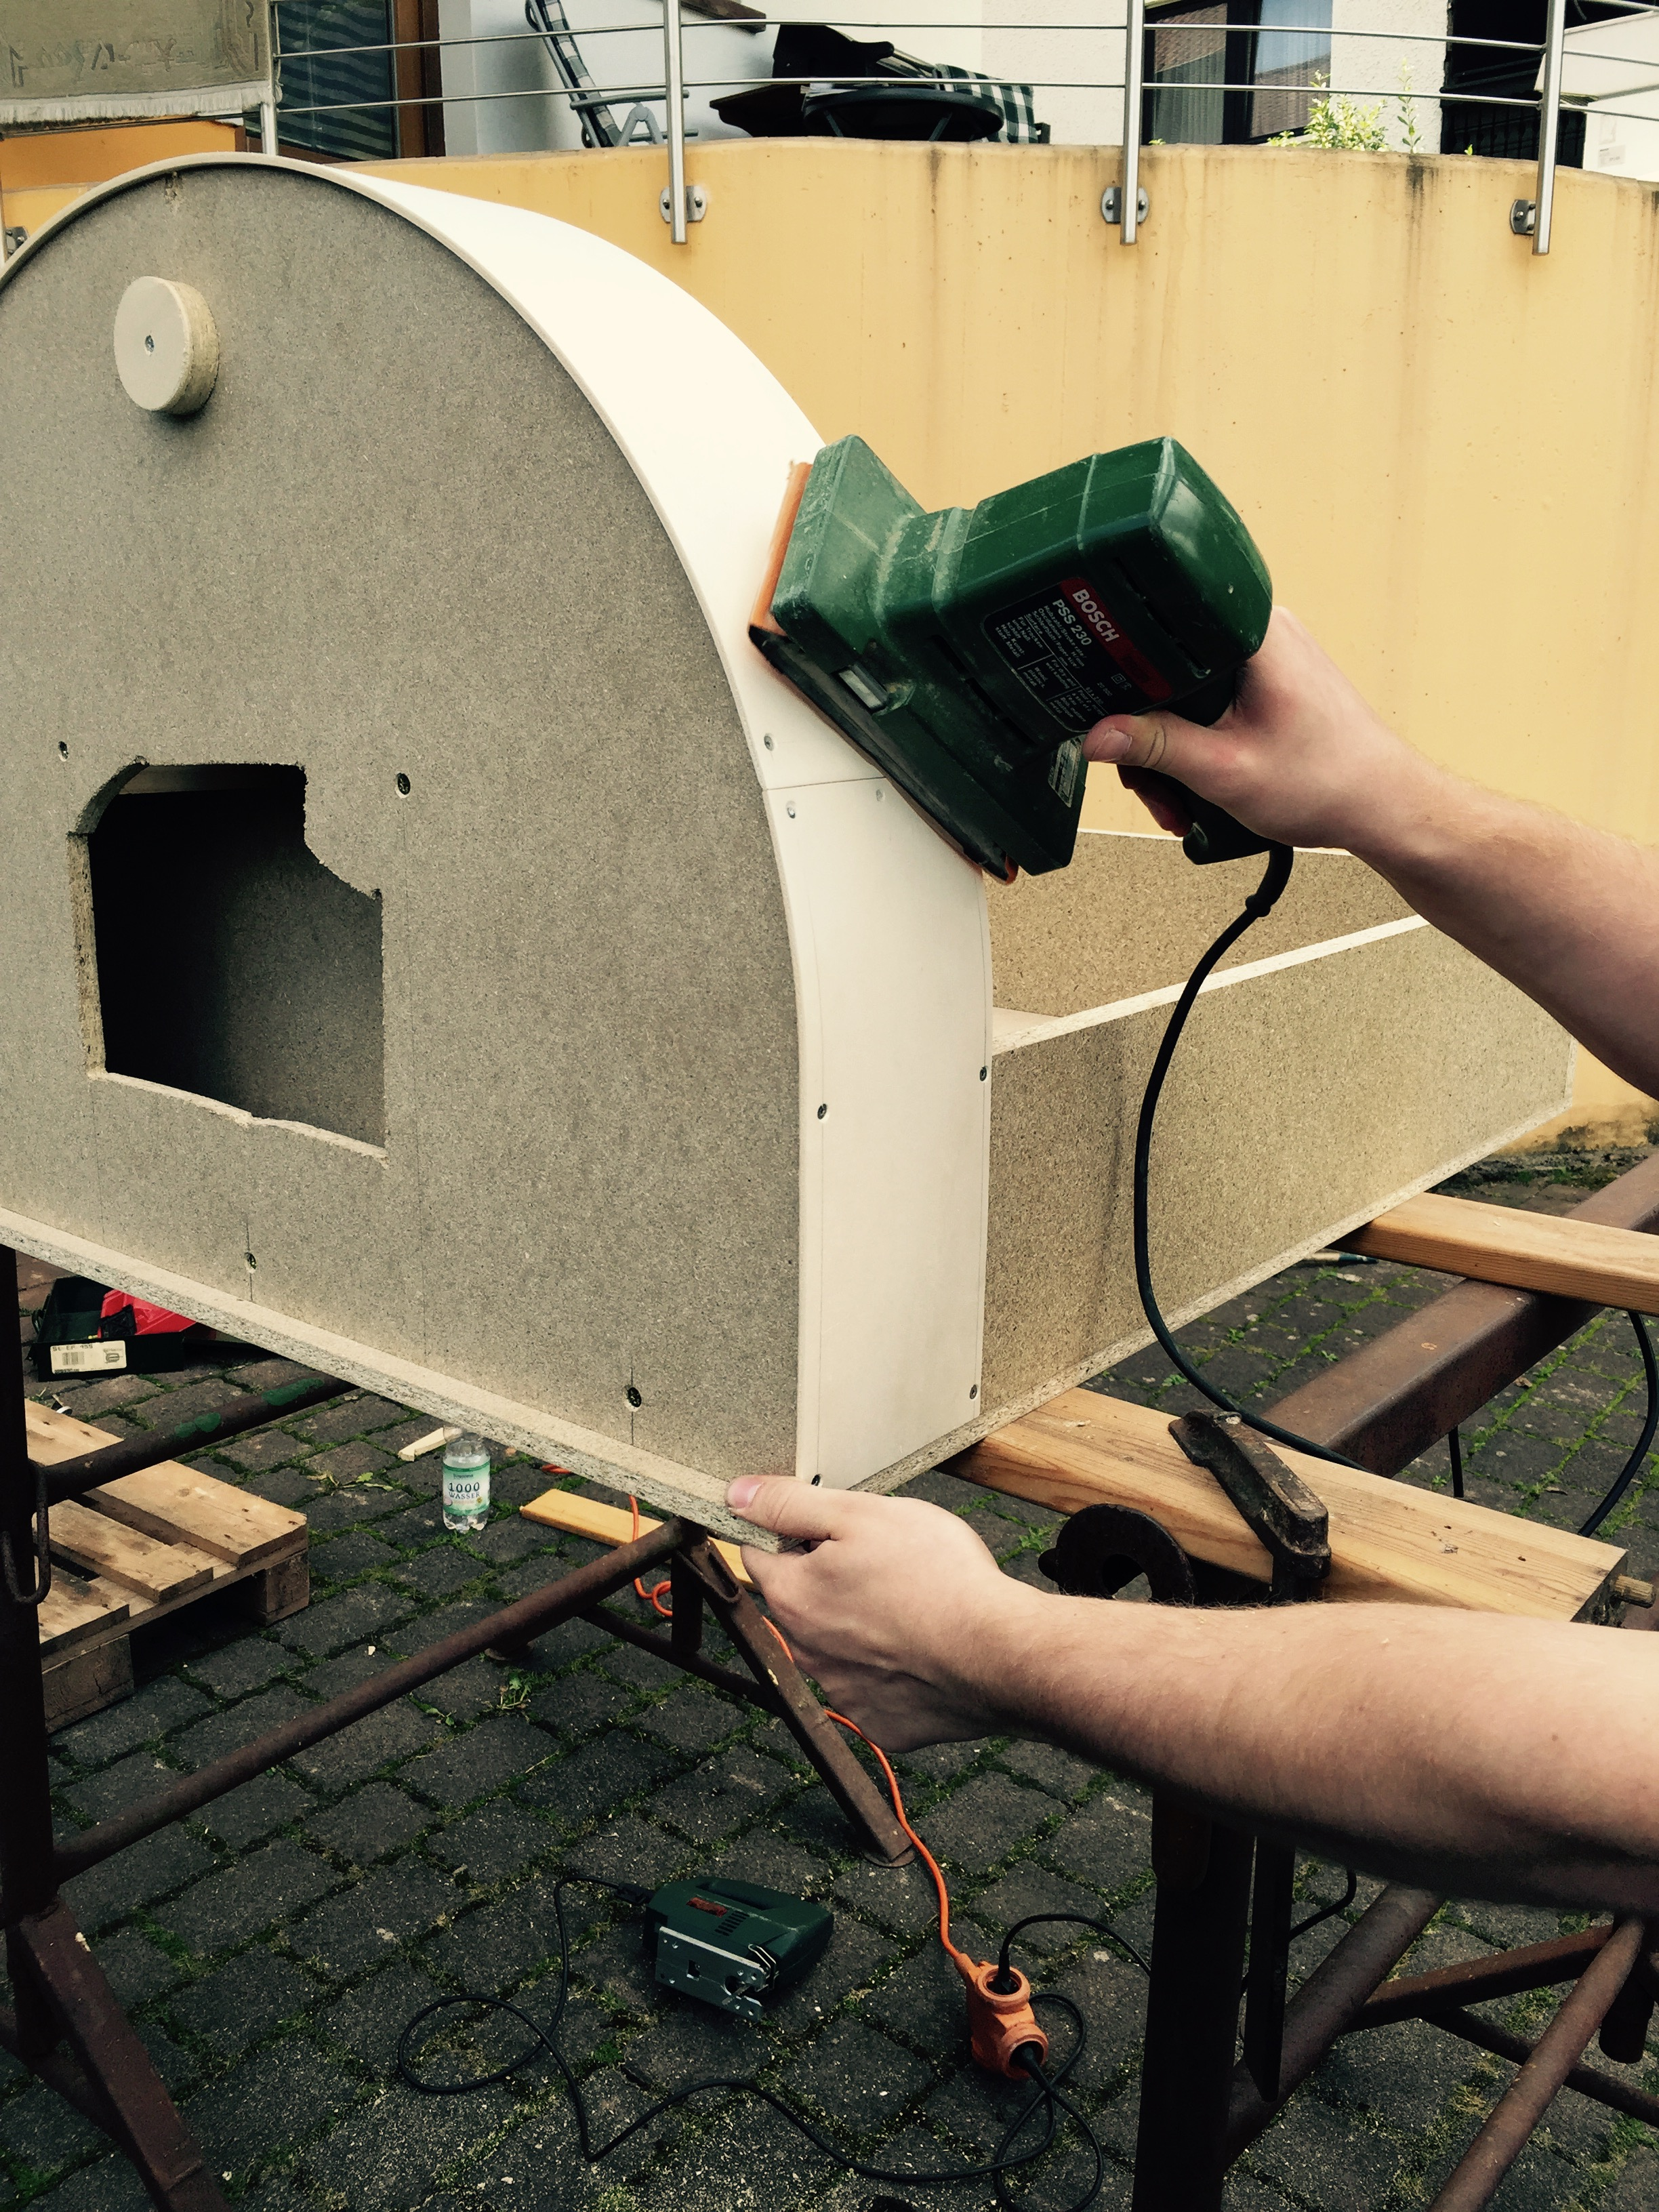
\includegraphics[width=0.5\linewidth]{pictures/polishing.jpg}
  \caption{Polishing the rack}
  \label{fig:polishing}
\end{figure}

After polishing and cleaning the rack with compressed air, we were able to prime the rack. This is important since primer creates a smooth and consistent layer for the paint.

\begin{figure}[htbp] 
  \centering
     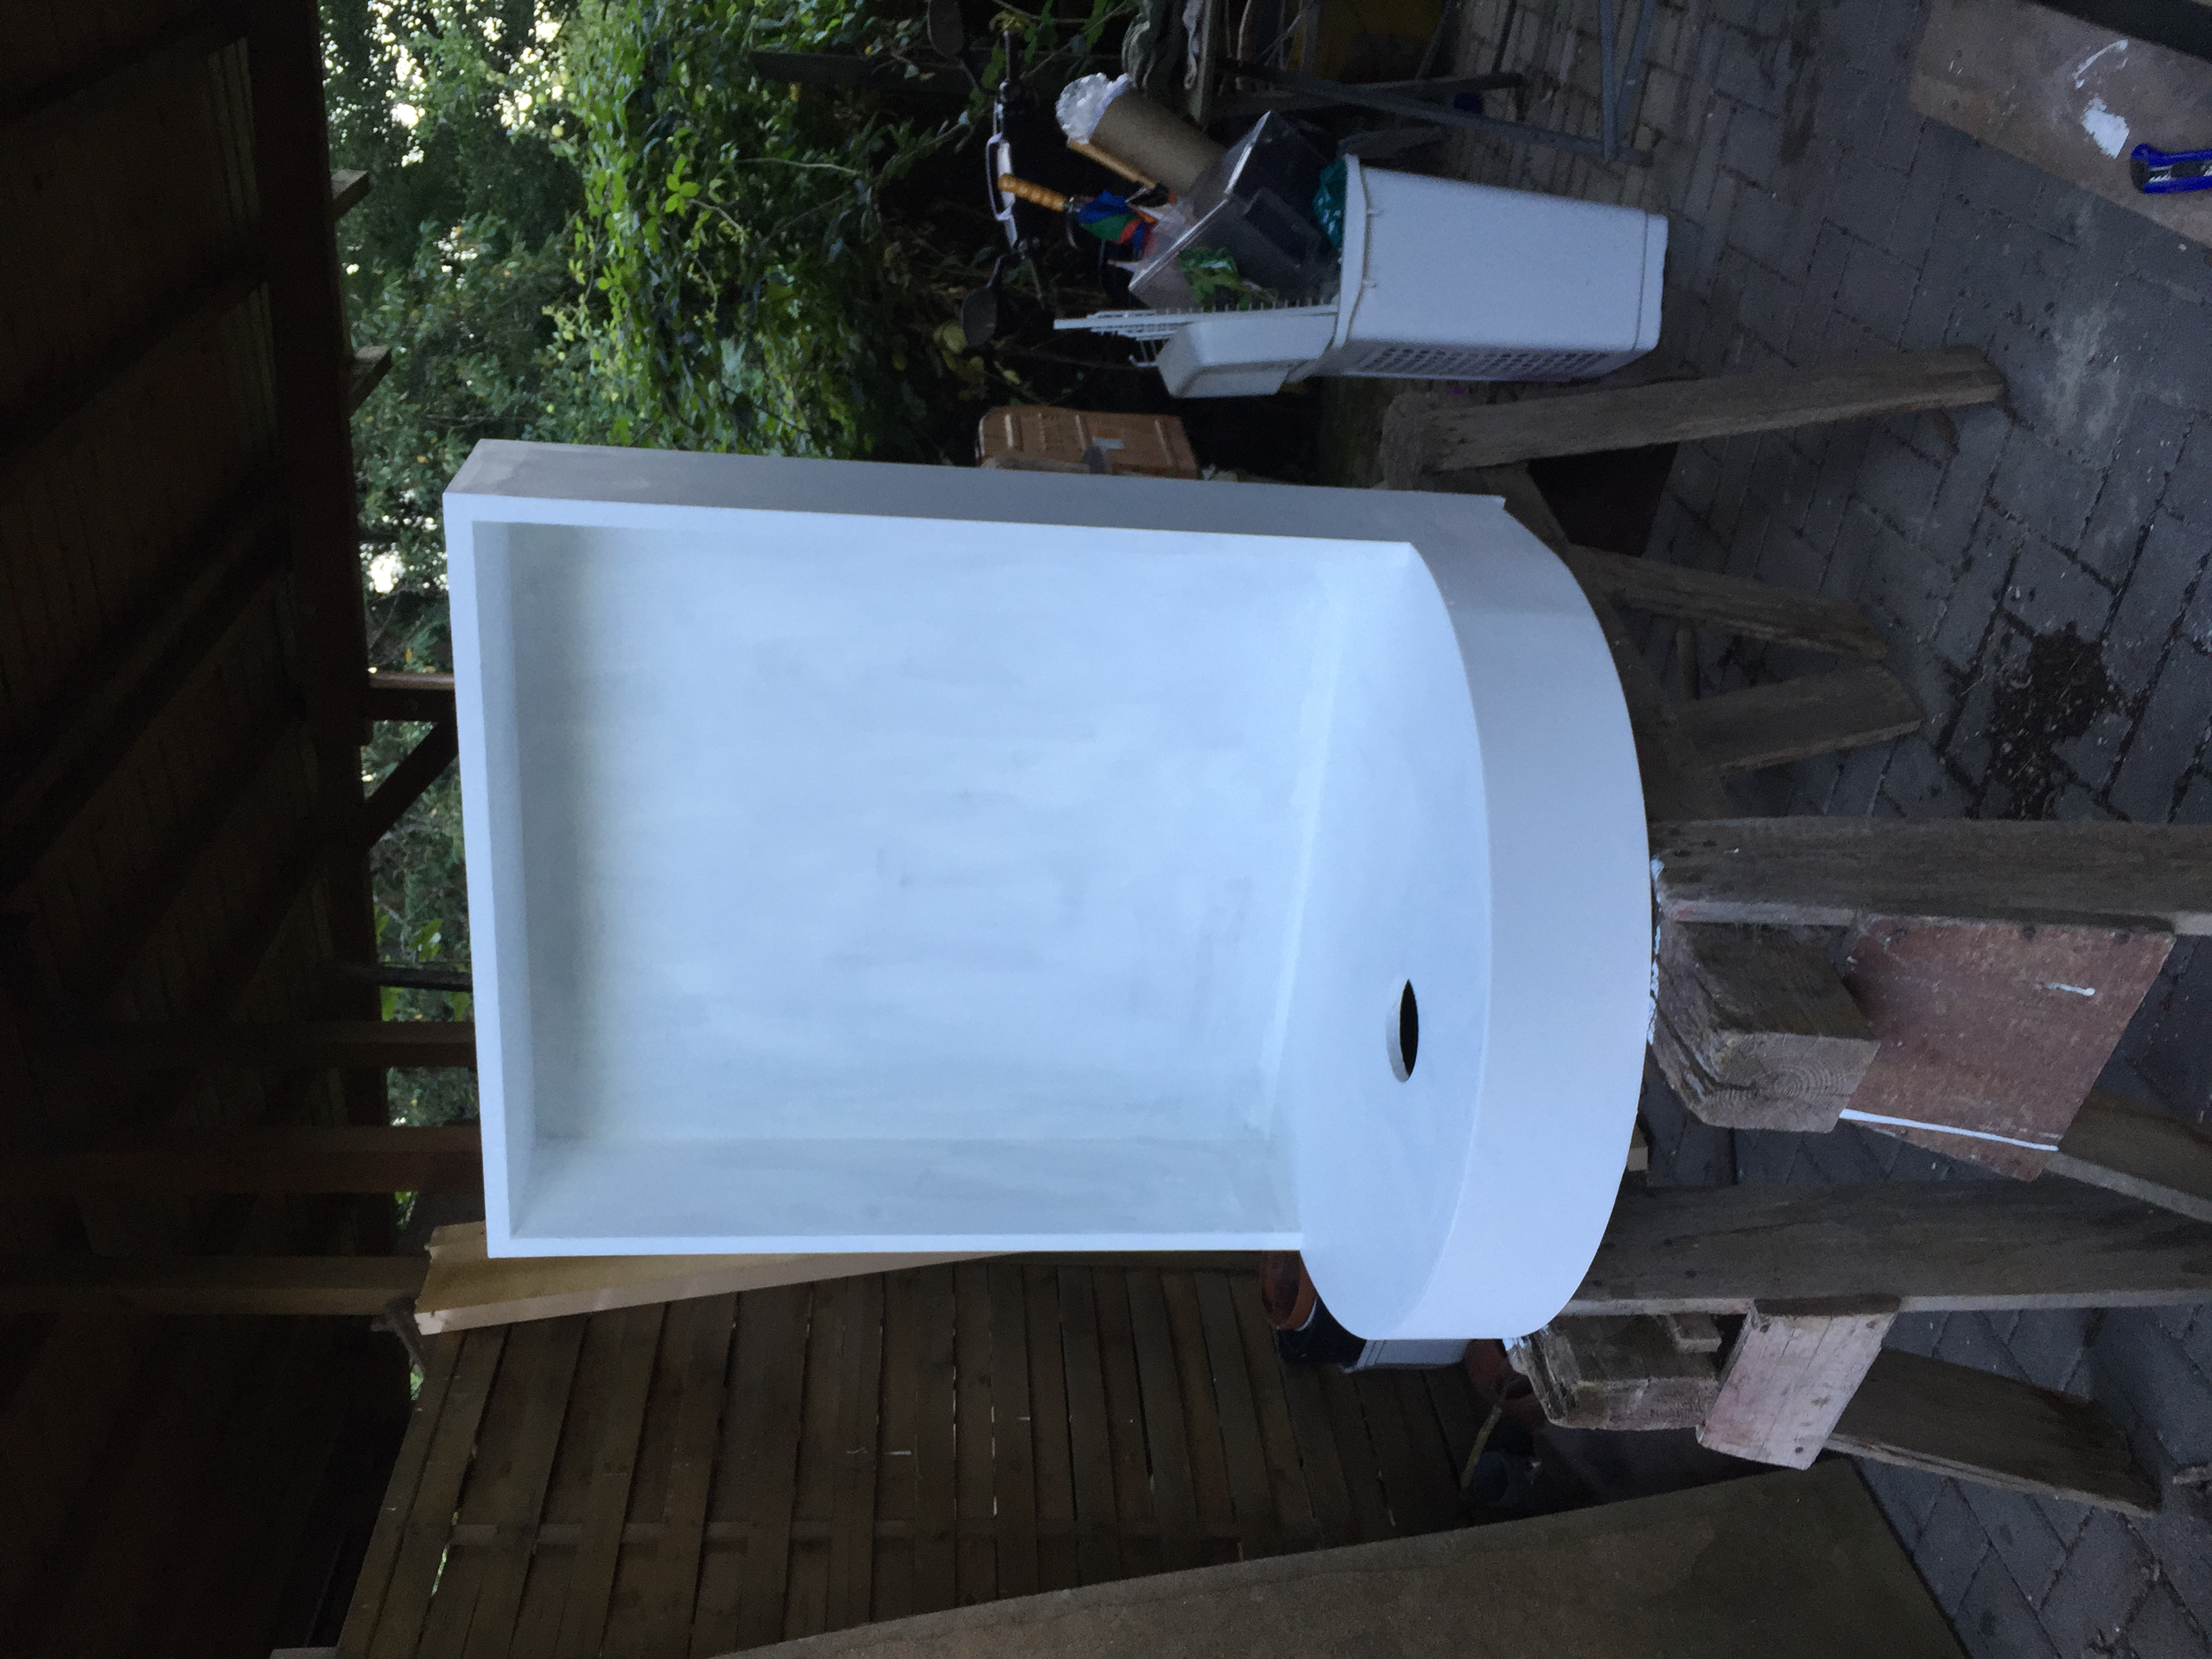
\includegraphics[width=0.6\linewidth, angle =270]{pictures/rack3.jpg}
  \caption{The primed rack}
  \label{fig:priming}
\end{figure}



\subsection{Acrylic Glass}

\begin{figure}[htbp] 
  \centering
     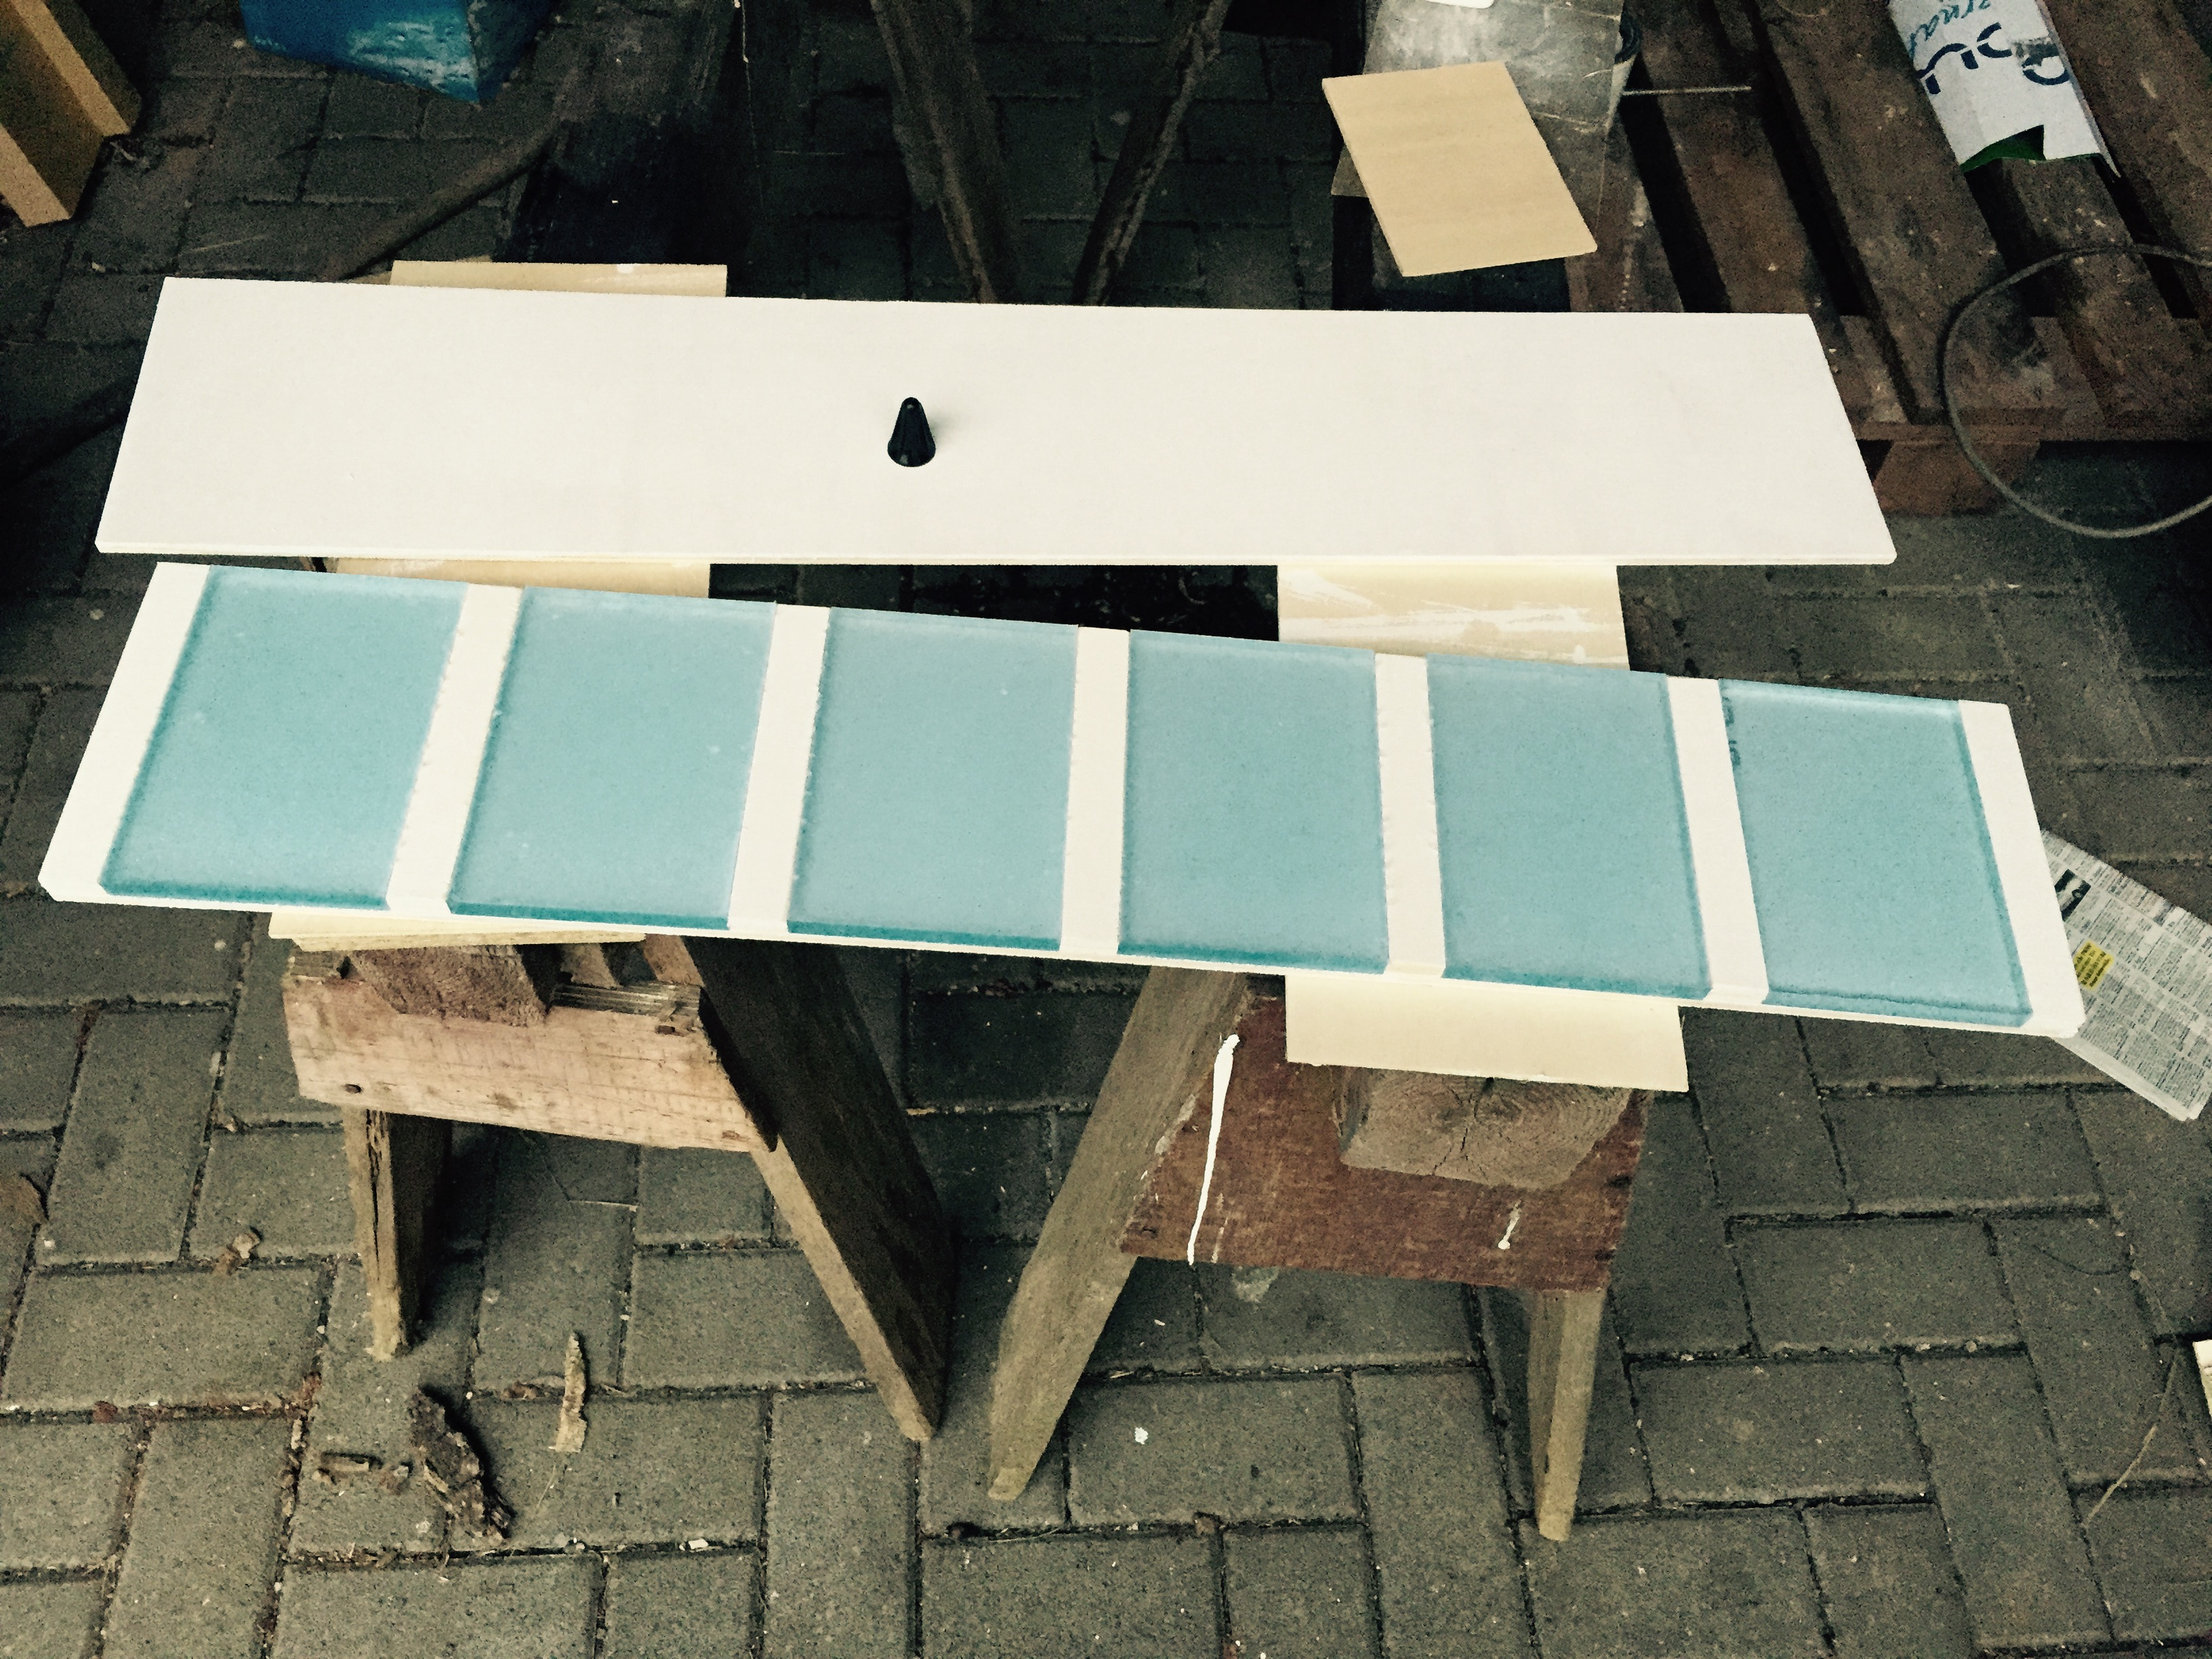
\includegraphics[width=0.5\linewidth]{pictures/plexiglass.jpg}
  \caption{Building the shelves}
  \label{fig:building_shelves}
\end{figure}

\begin{figure}[htbp] 
  \centering
     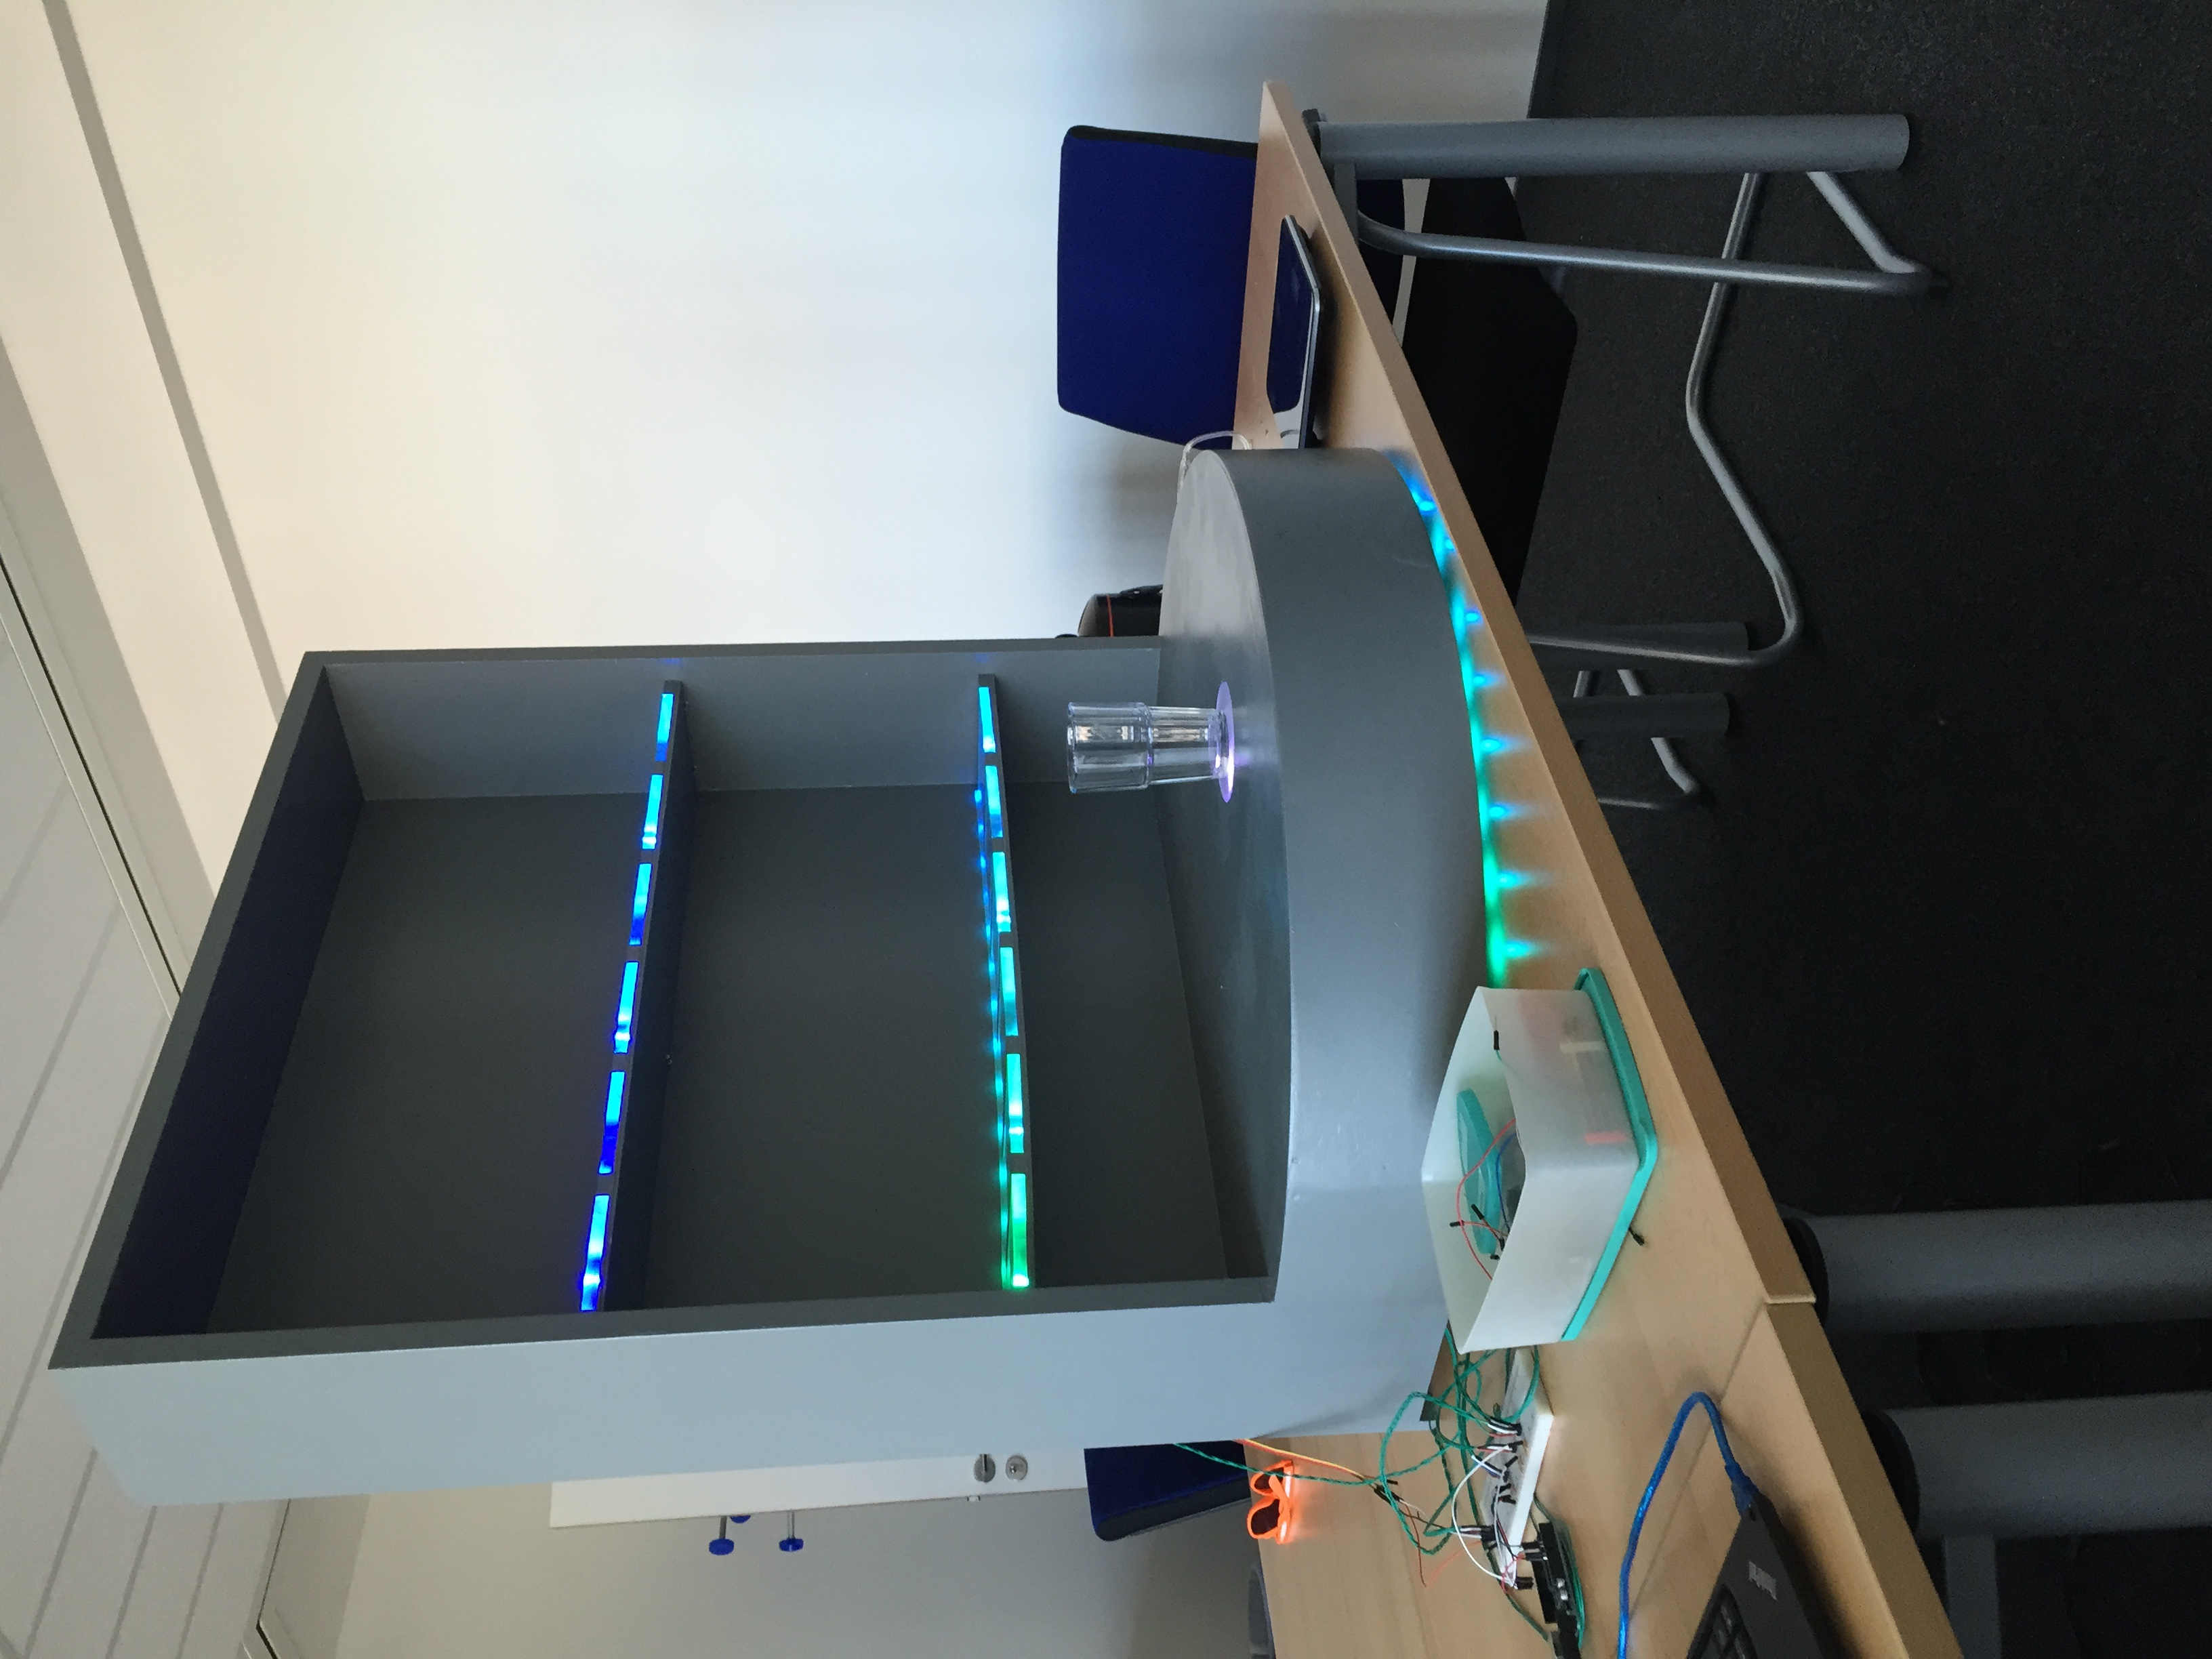
\includegraphics[width=0.5\linewidth]{pictures/iluminated_shelves.jpg}
  \caption{Building the shelves}
  \label{fig:iluminated_shelves}
\end{figure}


\subsection{Soldering and Wiring}
\section{Software Construction}
\subsection{Raspberry Pi and Arduino}
\subsection{Webserver}
\subsection{Database}
\subsection{Communication}
\section{User Guide}
\subsection{Start the System}
\subsection{Select a Cocktail}
\subsection{Mix the Cocktail}


\section{Conclusions}
%This paragraph will end the body of this sample document.
%Remember that you might still have Acknowledgments or
%Appendices; brief samples of these
%follow.  There is still the Bibliography to deal with; and
%we will make a disclaimer about that here: with the exception
%of the reference to the \LaTeX\ book, the citations in
%this paper are to articles which have nothing to
%do with the present subject and are used as
%examples only.
%\end{document}  % This is where a 'short' article might terminate

%ACKNOWLEDGMENTS are optional
%\section{Acknowledgments}
%This section is optional; it is a location for you
%to acknowledge grants, funding, editing assistance and
%what have you.  In the present case, for example, the
%authors would like to thank Gerald Murray of ACM for
%his help in codifying this \textit{Author's Guide}
%and the \textbf{.cls} and \textbf{.tex} files that it describes.
%
%%
%% The following two commands are all you need in the
%% initial runs of your .tex file to
%% produce the bibliography for the citations in your paper.
%\bibliographystyle{abbrv}
%\bibliography{sigproc}  % sigproc.bib is the name of the Bibliography in this case
%% You must have a proper ".bib" file
%%  and remember to run:
%% latex bibtex latex latex
%% to resolve all references
%%
%% ACM needs 'a single self-contained file'!
%%
%%APPENDICES are optional
%%\balancecolumns
%\appendix
%%Appendix A
%\section{Headings in Appendices}
%The rules about hierarchical headings discussed above for
%the body of the article are different in the appendices.
%In the \textbf{appendix} environment, the command
%\textbf{section} is used to
%indicate the start of each Appendix, with alphabetic order
%designation (i.e. the first is A, the second B, etc.) and
%a title (if you include one).  So, if you need
%hierarchical structure
%\textit{within} an Appendix, start with \textbf{subsection} as the
%highest level. Here is an outline of the body of this
%document in Appendix-appropriate form:
%\subsection{Introduction}
%\subsection{The Body of the Paper}
%\subsubsection{Type Changes and  Special Characters}
%\subsubsection{Math Equations}
%\paragraph{Inline (In-text) Equations}
%\paragraph{Display Equations}
%\subsubsection{Citations}
%\subsubsection{Tables}
%\subsubsection{Figures}
%\subsubsection{Theorem-like Constructs}
%\subsubsection*{A Caveat for the \TeX\ Expert}
%\subsection{Conclusions}
%\subsection{Acknowledgments}
%\subsection{Additional Authors}
%This section is inserted by \LaTeX; you do not insert it.
%You just add the names and information in the
%\texttt{{\char'134}additionalauthors} command at the start
%of the document.
%\subsection{References}
%Generated by bibtex from your ~.bib file.  Run latex,
%then bibtex, then latex twice (to resolve references)
%to create the ~.bbl file.  Insert that ~.bbl file into
%the .tex source file and comment out
%the command \texttt{{\char'134}thebibliography}.
%% This next section command marks the start of
%% Appendix B, and does not continue the present hierarchy
%\section{More Help for the Hardy}
%The acm\_proc\_article-sp document class file itself is chock-full of succinct
%and helpful comments.  If you consider yourself a moderately
%experienced to expert user of \LaTeX, you may find reading
%it useful but please remember not to change it.
%\balancecolumns
% That's all folks!
\end{document}
